%\documentclass[12pt,serif]{beamer}
%\documentclass[tikz,12pt,svgnames]{beamer}

%For printing
%\documentclass[table,handout,tikz,12pt,svgnames]{beamer}
%With animations
\documentclass[table,tikz,12pt,svgnames]{beamer}

\usepackage{CM-preamble}
\usepackage{gitdags}
\usepackage{subcaption}
 
\title{\LARGE Gestion de versions}
\subtitle{avec \texttt{git}}
\date{}

%README TODO STUFF

\begin{document}

\begin{frame}
	\titlepage
\end{frame}

\begin{frame}
	\frametitle{Moi... \textit{\small (et ma décharge de responsabilité)}}
	\begin{itemize}
		\item Je suis étranger (hors UE)…
		\item J'ai un accent…
		\item Je me {\color{blue} trompe beaucoup} en français
		\begin{itemize}
			\item et en info, et en math, et \ldots
			\item n'hésitez pas à me corriger ou à me demander de répéter
		\end{itemize}
		\item Je commence à enseigner
		\begin{itemize}
			\item ce cours est tout nouveau
			\item j'accepte des critiques (constructives mais pas que)\\
			et surtout des recommandations
			\item n'hésitez pas à poser des questions
		\end{itemize}
	\end{itemize}
\end{frame}


\begin{frame}
	\frametitle{Comment gérez-vous vos fichiers ? }
	\vspace{-1em}
	\begin{block}{}<1->
	\begin{itemize}
		\item Garder l'historique
		\item Partager
	\end{itemize}
	\end{block}
	\vspace{-2em}
	\begin{block}{}<2->
    \begin{adjustwidth}{-0.5cm}{}
		\begin{center}	
		{
\includegraphics[scale=0.5]{images/file_versions.pdf}}
		\end{center}
	\end{adjustwidth}
	\end{block}
\end{frame}



\begin{frame}
	\frametitle{Comment collaborer sur un fichier ? }
	\vspace{-1em}
	\begin{block}{}
    \begin{adjustwidth}{-0.5cm}{}
		\begin{center}
		{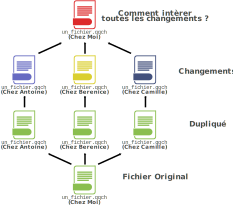
\includegraphics[scale=0.38]{images/file_share.pdf}}
		\end{center}
	\end{adjustwidth}
	\end{block}
\end{frame}


\begin{frame}
	\frametitle{Comment collaborer sur plusieurs fichiers ? }
%	\vspace{-4em}
	\begin{block}{}
    \begin{adjustwidth}{-0.5cm}{}
		\begin{center}
		{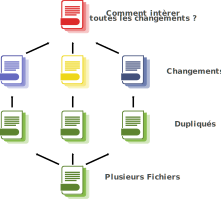
\includegraphics[scale=0.38]{images/file_share_many.pdf}}
		\end{center}
	\end{adjustwidth}
	\end{block}
\end{frame}


\begin{frame}
	\frametitle{D'autres solutions ? }
	\vspace{-4em}
	\begin{block}{}
    \begin{adjustwidth}{-0.5cm}{}
		\begin{center}
		{
\includegraphics[scale=0.43]{images/services.pdf}}
		\end{center}
	\end{adjustwidth}
	\end{block}
\end{frame}



\begin{frame}
	\frametitle{Gestion de versions}
		\begin{block}{}
%			\begin{itemize}
%				\item
				La \textbf{gestion de versions} (en anglais \textit{version control} ou \textit{revision control}) consiste à maintenir l'ensemble des versions d'un ou plusieurs fichiers (généralement en texte).
				Essentiellement utilisée dans le domaine de la création de logiciels, elle concerne surtout \textbf{la gestion des codes source}.
%			\end{itemize}
		\end{block}
		\begin{block}{}
		\small \url{https://fr.wikipedia.org/wiki/Gestion\_de\_versions}
		\end{block}
\end{frame}


\begin{frame}
	\frametitle{Gestion de versions}
	\vspace{-2em}
	\begin{block}{}
    \begin{adjustwidth}{-5.5cm}{}
		\begin{center}
		{\includegraphics[scale=0.58]{images/gestion_versions.pdf}}
		\end{center}
	\end{adjustwidth}
	\vspace{-4em}
    \begin{adjustwidth}{5.0cm}{}
	\tiny Par Revision\_controlled\_project\_visualization.svg: *Subversion\_project\_visualization.svg: Traced by User:Stannered, original by en:User:Sami Keroladerivative work: Moxfyre (talk)derivative work: Echion2 (talk) — Revision\_controlled\_project\_visualization.svg, CC BY-SA 3.0, \url{https://commons.wikimedia.org/w/index.php?curid=9562807}
	\end{adjustwidth}
	\end{block}
\end{frame}

\begin{frame}
	\frametitle{Avantages de la gestion de versions}
	\begin{block}{}
    \begin{adjustwidth}{-0.9cm}{}
		\begin{itemize}
			\item Sauvegarde / Restauration
			\item Synchronisation du travail (partage, collaboration)
			\item Suivi de changements (très détaillé)
			\item Suivi de responsabilités / propriétaires / coupables
			\item \textit{Sandboxing} (espace confiné, environnement de test, isolation)
			\item \textit{Branching and merging}
			\item Passage à l'échelle (10, 100, 1.000, 10.000 développeurs)
		\end{itemize}
	\end{adjustwidth}
	\end{block}
	\begin{block}{}
    \begin{adjustwidth}{-0.9cm}{}
		\begin{itemize}
%			\item Et pour les sauvegardes ? (\small\textit{pas vraiment})
		\end{itemize}
	\end{adjustwidth}
	\end{block}
\end{frame}

\begin{frame}
	\frametitle{Que mettre dans un Logiciel de Gestion de Versions ?}
	\vspace{-2em}
	\begin{block}{}%À mettre
    \begin{adjustwidth}{-0.5cm}{}
		\begin{itemize}
			\item Tous les sources du projet
			\begin{itemize}
				\item code source (\texttt{.c .cpp .java .py} \dots)
				\item scripts de build (\texttt{Makefile pom.xml} \ldots)
				\item Documentation (\texttt{.txt .tex Readme} \ldots)
				\item Ressources (images \ldots)
				\item Scripts divers (déploiement, \texttt{.sql, .sh} \ldots)
			\end{itemize}
		\end{itemize}
	\end{adjustwidth}	
	\end{block}
	\begin{block}{\color{red} À NE PAS mettre}<2->
    \begin{adjustwidth}{-0.5cm}{}
	\begin{itemize}
		\item Les fichiers générés
		\begin{itemize}
			\item Résultat de compilation (\texttt{.class .o .exe .jar} \ldots)
			\item Autres fichiers générés (\texttt{.ps .dvi .pdf javadoc} \ldots)
		\end{itemize}
	\end{itemize}
	\end{adjustwidth}
	\end{block}
\end{frame}


%\begin{frame}
%	\frametitle{TODO}
%	\begin{block}{}
%%    \begin{adjustwidth}{-0.9cm}{}
%		\begin{itemize}
%			\item Workflow from video
%			\item Workflow from video for sharing
%			\item Do the working directory, staging, repository image...
%			Then a collaboration immage, showing multiple copies of the repository...
%		\end{itemize}
%%	\end{adjustwidth}
%	\end{block}
%\end{frame}

\begin{frame}
\frametitle{TODO: BREAK INTO MULTIPLE IMAGES TO EXPLAIN EACH COMMAND}
\vspace{-2em}
\begin{block}{}
		\begin{center}
%			{\includegraphics[scale=0.55]{images/MgaV9.png}}
			{\includegraphics[scale=0.45]{images/MgaV9.png}}
		\end{center}
\end{block}
\end{frame}


%%%%%%%%%% Begin Premier Commit
\begin{frame}[fragile]
\frametitle{The Directed Acyclic \textit{Commit}-Graph in Git}
%	\vspace{-0.5cm}
 	\begin{figure}
	%\only<2->{
	\onslide<2>{
		\begin{subfigure}[h]{\textwidth}
		%\centering
		\begin{tikzpicture}
		% Commit DAG
		\gitDAG[grow right sep = 2em]{
			27ff4
		};
		% Tag reference
	%	\gittag [v0p1] {v0.1} {above=of A} {A}
		% Remote branch
		% Branch
		\gitbranch
		{master}     % node name and text 
		{above=of 27ff4} % node placement
		{27ff4}          % target
		% HEAD reference
		\gitHEAD
		%	 			{above=of master} % node placement
		{right=of master} % node placement
		{27ff4}          % target
		\end{tikzpicture}
		\end{subfigure}
	}	
	\subcaption{\only<1>{Dépôt vide}\only<2->{Premier \textit{commit}}}
	\end{figure}

%	\vspace{-0.5cm}
	\begin{block}{Dans un terminal \ldots}
	\vspace{-0.2cm}		
	\begin{minted}[mathescape=true,escapeinside=||,tabsize=4
	,fontsize=\footnotesize,
	]{bash}
	mkdir mon_depot ; cd mon_depot
	git init .
	echo "pomme" |>{}>| fruits.txt
	git add fruits.txt
	git commit -m "Pomme ajouté à la liste de fruits"
		===> ID = 27ff4
	\end{minted}
	\end{block}
	Faire \texttt{git status} et \texttt{git log} \underline{après chaque commande}!!!
\end{frame}
%%%%%%%%%% End Premier Commit

\begin{frame}
\frametitle{C'est quoi un commit ?}
	\vspace{-1em}
	\begin{block}{}
	\begin{adjustwidth}{-0.5cm}{}
		\begin{center}	
			{\includegraphics[scale=0.6]{images/git_commit.png}}
		\end{center}
	\end{adjustwidth}
	\end{block}

	\vspace{-2em}
	\begin{block}{}
	%    \begin{adjustwidth}{-0.9cm}{}
	\begin{itemize}
		\item Le \texttt{Commit-ID} est une \textit{empreinte} calculé en utilisant la fonction de hachage \texttt{SHA-1} sur
		\begin{itemize}
			\item \textbf{Tout} le contenu du commit + Date + Nom et email du commiteur + Message de log + ID du commit parent + \ldots
		\end{itemize}
	\end{itemize}
	%	\end{adjustwidth}
%	\begin{itemize}
%	\item 
	Propriété : \textbf{Unicité} quasi-universelle de l'\texttt{ID}
%	\begin{itemize}
%		\item Unicité universelle statistique de l'ID
%	\end{itemize}
%\end{itemize}
%	\end{adjustwidth}
\end{block}
\end{frame}


%%%%%%%%%%% ANIMATION Commit 2
\begin{frame}[fragile]
\frametitle{The DAG in Git : Commit 2}
\only<1-2>{
	\begin{figure}
		\begin{subfigure}[h]{\textwidth}
			%\centering
			\begin{tikzpicture}
			% Commit DAG
			\gitDAG[grow right sep = 2em]{
				27ff4
			};
			% Tag reference
			%	\gittag [v0p1] {v0.1} {above=of A} {A}
			% Remote branch
			% Branch
			\gitbranch
			{master}     % node name and text 
			{above=of 27ff4} % node placement
			{27ff4}          % target
			% HEAD reference
			\gitHEAD
			%	 			{above=of master} % node placement
			{right=of master} % node placement
			{27ff4}          % target
			\end{tikzpicture}
			\subcaption{État avant deuxième \texttt{commit}}
		\end{subfigure}
	\end{figure}
}

\only<3>{
	\begin{figure}
		\begin{subfigure}[h]{\textwidth}
			%\centering
			\begin{tikzpicture}
			% Commit DAG
			\gitDAG[grow right sep = 2em]{
				27ff4 -- 31490
			};
			% Tag reference
			%	\gittag [v0p1] {v0.1} {above=of A} {A}
			% Remote branch
			% Branch
			\gitbranch
			{master}     % node name and text 
			{above=of 31490} % node placement
			{31490}          % target
			% HEAD reference
			\gitHEAD
			%	 			{above=of master} % node placement
			{right=of master} % node placement
			{31490}          % target
			\end{tikzpicture}
			\subcaption{Deuxième \textit{commit}}
		\end{subfigure}
	\end{figure}
}

%\vspace{-0.5cm}
%\vspace{0.4cm} \begin{center} \noindent\makebox[\linewidth]{\line(2,0){500}} \end{center} \vspace{-0.4cm} 
\begin{block}{Dans un terminal \ldots}<2->
%	\vspace{-0.2cm}		
	\begin{minted}[mathescape=true,escapeinside=||,tabsize=4
	,fontsize=\footnotesize,
	]{bash}
	echo banane |>{}>| fruits.txt
	git add fruits.txt
	git commit -m "Ajouté banane à fruits.txt"
		===> ID = 31490
	\end{minted}
\end{block}
\end{frame}
%%%%%%%%%%% End ANIMATION Commit 2


%%%%%%%%%%% ANIMATION Commit 3
\begin{frame}[fragile]
\frametitle{The DAG in Git : Commit 3}

	\begin{figure}
		\begin{subfigure}[h]{\textwidth}
			%\centering
			\begin{tikzpicture}
			% Commit DAG
			\gitDAG[grow right sep = 2em]{
				27ff4 -- 31490 -- ab5d1
			};
			% Tag reference
			%	\gittag [v0p1] {v0.1} {above=of A} {A}
			% Remote branch
			% Branch
			\gitbranch
			{master}     % node name and text 
			{above=of ab5d1} % node placement
			{ab5d1}          % target
			% HEAD reference
			\gitHEAD
			%	 			{above=of master} % node placement
			{right=of master} % node placement
			{ab5d1}          % target
			\end{tikzpicture}
			\subcaption{Troisième \textit{commit}}
		\end{subfigure}
	\end{figure}

%\vspace{-0.5cm}
\begin{block}{}%Sur le terminal \ldots}
%	\vspace{-0.2cm}
	\vspace{0.4cm} \begin{center} \noindent\makebox[\linewidth]{\line(2,0){500}} \end{center} \vspace{-0.4cm} 		
	\begin{minted}[mathescape=true,escapeinside=||,tabsize=4,fontsize=\footnotesize,linenos,
	]{bash}
	echo orange |>{}>| fruits.txt
	git add fruits.txt
	git commit -m "Ajouté orange à fruits.txt"
		===> ID = ab5d1
	\end{minted}
\end{block}
\end{frame}
%%%%%%%%%%% End ANIMATION Commit 3


%%%%%%%%%%% ANIMATION Branch 1
\begin{frame}[fragile]
\frametitle{The DAG in Git: Branches 1}
\only<1-2>{
	\begin{figure}
	\begin{subfigure}[h]{\textwidth}
		%\centering
		\begin{tikzpicture}
		% Commit DAG
		\gitDAG[grow right sep = 2em]{
			27ff4 -- 31490 -- ab5d1
		};
		% Tag reference
		%	\gittag [v0p1] {v0.1} {above=of A} {A}
		% Remote branch
		% Branch
		\gitbranch
		{master}     % node name and text 
		{above=of ab5d1} % node placement
		{ab5d1}          % target
		% HEAD reference
		\gitHEAD
		%	 			{above=of master} % node placement
		{right=of master} % node placement
		{ab5d1}          % target
		\end{tikzpicture}
		\subcaption{Avant branche}
	\end{subfigure}
	\end{figure}
}

\only<3-4>{
	\begin{figure}
	\begin{subfigure}[h]{\textwidth}
		%\centering
		\begin{tikzpicture}
		% Commit DAG
		\gitDAG[grow right sep = 2em]{
			27ff4 -- 31490 -- ab5d1
		};
		% Tag reference
		%	\gittag [v0p1] {v0.1} {above=of A} {A}
		% Remote branch
		% Branch
		\gitbranch
		{master}     % node name and text 
		{above=of ab5d1} % node placement
		{ab5d1}          % target
		% HEAD reference
		\gitHEAD
		%	 			{above=of master} % node placement
		{right=of master} % node placement
		{ab5d1}          % target
		\gitbranch {legumes} {left=of master} {ab5d1}

		\end{tikzpicture}
		\subcaption{Après branche}
		\only<3>{==> une nouvelle \textit{étiquette} apparait}
	\end{subfigure}
\end{figure}
}

\only<5-6>{
	\begin{figure}
		\begin{subfigure}[h]{\textwidth}
			%\centering
			\begin{tikzpicture}
			% Commit DAG
			\gitDAG[grow right sep = 2em]{
				27ff4 -- 31490 -- ab5d1 -- ffd5c
			};
			% Tag reference
			%	\gittag [v0p1] {v0.1} {above=of A} {A}
			% Remote branch
			% Branch
			\gitbranch
			{master}     % node name and text 
			{above=of ab5d1} % node placement
			{ab5d1}          % target
			% HEAD reference
			\gitHEAD
 			{below=of ffd5c} % node placement
%			{right=of legumes} % node placement
			{ffd5c}          % target
			\gitbranch {legumes} {above=of ffd5c} {ffd5c}
			
			\end{tikzpicture}
			\subcaption{Après commit dans branche \texttt{legumes}}
			\only<3>{==> une nouvelle \textit{étiquette} apparait}
		\end{subfigure}
	\end{figure}
}

\only<7->{
	\begin{figure}
		\begin{subfigure}[h]{\textwidth}
			%\centering
			\begin{tikzpicture}
			% Commit DAG
			\gitDAG[grow right sep = 2em]{
				27ff4 -- 31490 -- ab5d1 -- ffd5c -- 8a928
			};
			% Tag reference
			%	\gittag [v0p1] {v0.1} {above=of A} {A}
			% Remote branch
			% Branch
			\gitbranch
			{master}     % node name and text 
			{above=of ab5d1} % node placement
			{ab5d1}          % target
			% HEAD reference
			\gitHEAD
			{below=of 8a928} % node placement
			%			{right=of legumes} % node placement
			{8a928}          % target
			\gitbranch {legumes} {above=of 8a928} {8a928}
			
			\end{tikzpicture}
			\subcaption{Après deuxième commit dans branche \texttt{legumes}}
			\only<3>{==> une nouvelle \textit{étiquette} apparait}
		\end{subfigure}
	\end{figure}
}

%\vspace{-0.5cm}
%\only<2-3>{
%\begin{block}{Sur le terminal \ldots}
	\pause[2]
	\vspace{0.4cm} \begin{center} \noindent\makebox[\linewidth]{\line(2,0){500}} \end{center} \vspace{-0.4cm}
	\begin{minted}[mathescape=true,escapeinside=||,tabsize=4,fontsize=\footnotesize,]{bash}
	git branch legumes ; git checkout legumes
	\end{minted}
	\pause[4]
	\begin{minted}[mathescape=true,escapeinside=||,tabsize=4,fontsize=\footnotesize,]{bash}
	echo auvergine |>{}>| legumes.txt ; git add legumes.txt
	git commit -m "Ajout auvergine à legumes"
		===> ID = ffd5c
	\end{minted}
	\pause[6]
	\begin{minted}[mathescape=true,escapeinside=||,tabsize=4,fontsize=\footnotesize,]{bash}
	echo courgette |>{}>| legumes.txt ; git add legumes.txt
	git commit -m "Ajout courgette à legumes"
		===> ID = 8a928
	\end{minted}
\end{frame}
%%%%%%%%%%% End ANIMATION Branch 1
%echo auvergine |>{}>| legumes.txt
%echo courgette |>{}>| legumes.txt
%git add legumes.txt
%git commit -m "Ajout de legumes"
%===> ID = ffd5c	



%%%%%%%%%%% ANIMATION Branch 2
\begin{frame}[fragile]
\frametitle{The DAG in Git: Branches 2}
\only<1>{
	\begin{figure}
		\begin{subfigure}[h]{\textwidth}
			%\centering
			\begin{tikzpicture}
			% Commit DAG
			\gitDAG[grow right sep = 2em]{
				27ff4 -- 31490 -- ab5d1 -- ffd5c -- 8a928
			};
			% Tag reference
			%	\gittag [v0p1] {v0.1} {above=of A} {A}
			% Remote branch
			% Branch
			\gitbranch
			{master}     % node name and text 
			{above=of ab5d1} % node placement
			{ab5d1}          % target
			% HEAD reference
			\gitHEAD
			{below=of 8a928} % node placement
			%			{right=of legumes} % node placement
			{8a928}          % target
			\gitbranch {legumes} {above=of 8a928} {8a928}
			
			\end{tikzpicture}
			\subcaption{Travaillons sur \texttt{master}}
			\only<2>{$\Longrightarrow$ \texttt{legumes.txt} n'existe plus dans \textit{Working Directory})}
		\end{subfigure}
	\end{figure}
}

\only<2-3>{
	\begin{figure}
		\begin{subfigure}[h]{\textwidth}
			%\centering
			\begin{tikzpicture}
			% Commit DAG
			\gitDAG[grow right sep = 2em]{
				27ff4 -- 31490 -- ab5d1 -- ffd5c -- 8a928
			};
			% Tag reference
			%	\gittag [v0p1] {v0.1} {above=of A} {A}
			% Remote branch
			% Branch
			\gitbranch
			{master}     % node name and text 
			{above=of ab5d1} % node placement
			{ab5d1}          % target
			% HEAD reference
			\gitHEAD
			{below=of ab5d1} % node placement
			%			{right=of legumes} % node placement
			{ab5d1}          % target
			\gitbranch {legumes} {above=of 8a928} {8a928}
			
			\end{tikzpicture}
			\subcaption{Travaillons sur \texttt{master}}
			\only<2>{$\Longrightarrow$ \texttt{legumes.txt} n'existe plus dans \textit{Working Directory})}
		\end{subfigure}
	\end{figure}
}

\only<4>{
	\begin{figure}
		\begin{subfigure}[h]{\textwidth}
			%\centering
			\begin{tikzpicture}
			% Commit DAG
			\gitDAG[grow right sep = 2em]{
				27ff4 -- 31490 -- ab5d1 -- {ffd5c -- 8a928, 21721}
			};
			% Tag reference
			%	\gittag [v0p1] {v0.1} {above=of A} {A}
			% Remote branch
			% Branch
			\gitbranch
			{master}     % node name and text 
			{below=of 21721} % node placement
			{21721}          % target
			% HEAD reference
			\gitHEAD
			{right=of master} % node placement
			%			{right=of legumes} % node placement
			{21721}          % target
			\gitbranch {legumes} {above=of 8a928} {8a928}
			
			\end{tikzpicture}
			\subcaption{Après nouveau \textit{commit} sur \texttt{master}}
			\only<2>{$\Longrightarrow$ \texttt{legumes.txt} n'existe plus dans \textit{Working Directory})}
		\end{subfigure}
	\end{figure}
}

%\vspace{-0.5cm}
%\only<2-3>{
%\begin{block}{Sur le terminal \ldots}
%\pause[2]
%\vspace{-0.2cm}
\vspace{0.4cm} \begin{center} \noindent\makebox[\linewidth]{\line(2,0){500}} \end{center} \vspace{-0.4cm}
\begin{minted}[mathescape=true,escapeinside=||,tabsize=4,fontsize=\footnotesize,]{bash}
	git checkout master
\end{minted}
\pause[3]
\begin{minted}[mathescape=true,escapeinside=||,tabsize=4,fontsize=\footnotesize,]{bash}
	echo poire |>{}>| fruits.txt ; git add fruits.txt
	git commit -m "Ajouté poire à fruits.txt"
		===> ID = 21721
\end{minted}
\end{frame}
%%%%%%%%%%% End ANIMATION Branch 2


%%%%%%%%%%% ANIMATION Merge 1
\begin{frame}[fragile]
\frametitle{The DAG in Git: Merge 1}
\only<1-2>{
	\begin{figure}
		\begin{subfigure}[h]{\textwidth}
			%\centering
			\begin{tikzpicture}
			% Commit DAG
			\gitDAG[grow right sep = 1.5em]{
				27ff4 -- 31490 -- ab5d1 -- {ffd5c -- 8a928, 21721}
			};
			% Tag reference
			%	\gittag [v0p1] {v0.1} {above=of A} {A}
			% Remote branch
			% Branch
			\gitbranch
			{master}     % node name and text 
			{below=of 21721} % node placement
			{21721}          % target
			% HEAD reference
			\gitHEAD
			{right=of legumes} % node placement
			%			{right=of legumes} % node placement
			{8a928}          % target
			\gitbranch {legumes} {above=of 8a928} {8a928}
			
			\end{tikzpicture}
			\subcaption{Allons sur \texttt{légumes}, regardons les différences}
			%\only<2>{$\Longrightarrow$ \texttt{legumes.txt} n'existe plus dans \textit{Working Directory})}
		\end{subfigure}
	\end{figure}
}

\only<3>{
	\begin{figure}
		\begin{subfigure}[h]{\textwidth}
			%\centering
			\begin{tikzpicture}
			% Commit DAG
			\gitDAG[grow right sep = 1.5em]{
				27ff4 -- 31490 -- ab5d1 -- {ffd5c -- 8a928, 21721} -- 760cf
			};
			% Tag reference
			%	\gittag [v0p1] {v0.1} {above=of A} {A}
			% Remote branch
			% Branch
			\gitbranch
			{master}     % node name and text 
			{below=of 21721} % node placement
			{21721}          % target
			% HEAD reference
			\gitHEAD
			{above=of 760cf} % node placement
			%			{right=of legumes} % node placement
			{760cf}          % target
			\gitbranch {legumes} {left=of gitHEAD} {760cf}
			
			\end{tikzpicture}
			\subcaption{Merger \texttt{master} dans \texttt{légumes} : produit un \underline{nouveau commit}}
			%\only<2>{$\Longrightarrow$ \texttt{legumes.txt} n'existe plus dans \textit{Working Directory})}
		\end{subfigure}
	\end{figure}
}


%\vspace{-0.5cm}
%\only<2-3>{
%\begin{block}{Sur le terminal \ldots}
%\pause[2]
%\vspace{-0.2cm}
\vspace{0.4cm} \begin{center} \noindent\makebox[\linewidth]{\line(2,0){500}} \end{center} \vspace{-0.4cm}
\begin{minted}[mathescape=true,escapeinside=||,tabsize=4,fontsize=\footnotesize,]{bash}
git checkout legumes
\end{minted}
\pause[2]
\begin{minted}[mathescape=true,escapeinside=||,tabsize=4,fontsize=\footnotesize,]{bash}
git diff master
\end{minted}
\pause[3]
\begin{minted}[mathescape=true,escapeinside=||,tabsize=4,fontsize=\footnotesize,]{bash}
git merge master
\end{minted}
\end{frame}
%%%%%%%%%%% End ANIMATION Merge 1

\begin{frame}
\frametitle{Merge 1 : Vue dans la console}
%\begin{block}{Représentation par pointeurs}%Parcours postfixé ou \texttt{GRD}}
\begin{adjustwidth}{-0.8cm}{}
	\begin{center}
		{\includegraphics[scale=0.3]{images/git_log_merge.png}}
	\end{center}
\end{adjustwidth}
%\end{block}
\end{frame}



%%%%%%%%%%% ANIMATION Merge 2
\begin{frame}[fragile]
\frametitle{The DAG in Git: Merge 2}
\only<1>{
	\begin{figure}
		\begin{subfigure}[h]{\textwidth}
			%\centering
			\begin{tikzpicture}
			% Commit DAG
			\gitDAG[grow right sep = 1.5em]{
				27ff4 -- 31490 -- ab5d1 -- {ffd5c -- 8a928, 21721} -- 760cf
			};
			% Tag reference
			%	\gittag [v0p1] {v0.1} {above=of A} {A}
			% Remote branch
			% Branch
			\gitbranch
			{master}     % node name and text 
			{below=of 21721} % node placement
			{21721}          % target
			% HEAD reference
			\gitHEAD
			{right=of master} % node placement
			%			{right=of legumes} % node placement
			{21721}          % target
			\gitbranch {legumes} {above=of 760cf} {760cf}
			
			\end{tikzpicture}
			\subcaption{Allons sur \texttt{master}}
			%\only<2>{$\Longrightarrow$ \texttt{legumes.txt} n'existe plus dans \textit{Working Directory})}
		\end{subfigure}
	\end{figure}
}

\only<2>{
	\begin{figure}
		\begin{subfigure}[h]{\textwidth}
			%\centering
			\begin{tikzpicture}
			% Commit DAG
			\gitDAG[grow right sep = 1.5em]{
				27ff4 -- 31490 -- ab5d1 -- {ffd5c -- 8a928, 21721} -- 760cf
			};
			% Tag reference
			%	\gittag [v0p1] {v0.1} {above=of A} {A}
			% Remote branch
			% Branch
			\gitbranch
			{master}     % node name and text 
			{below=of 760cf} % node placement
			{760cf}          % target
			% HEAD reference
			\gitHEAD
			{left=of legumes} % node placement
			%			{right=of legumes} % node placement
			{760cf}          % target
			\gitbranch {legumes} {above=of 760cf} {760cf}
			
			\end{tikzpicture}
			\subcaption{Merger \texttt{légumes} dans \texttt{master} : \underline{pas de nouveau commit}}
			%\only<2>{$\Longrightarrow$ \texttt{legumes.txt} n'existe plus dans \textit{Working Directory})}
		\end{subfigure}
	\end{figure}
}

\only<3>{
	\begin{figure}
		\begin{subfigure}[h]{\textwidth}
			%\centering
			\begin{tikzpicture}
			% Commit DAG
			\gitDAG[grow right sep = 1.5em]{
				27ff4 -- 31490 -- ab5d1 -- {ffd5c -- 8a928, 21721} -- 760cf
			};
			% Tag reference
			%	\gittag [v0p1] {v0.1} {above=of A} {A}
			% Remote branch
			% Branch
			\gitbranch
			{master}     % node name and text 
			{below=of 760cf} % node placement
			{760cf}          % target
			% HEAD reference
			\gitHEAD
			{above=of 760cf} % node placement
			%			{right=of legumes} % node placement
			{760cf}          % target
%			\gitbranch {legumes} {above=of 760cf} {760cf}
			
			\end{tikzpicture}
			\subcaption{Effacer la branche \texttt{légumes}}
			%\only<2>{$\Longrightarrow$ \texttt{legumes.txt} n'existe plus dans \textit{Working Directory})}
		\end{subfigure}
	\end{figure}
}
\vspace{0.4cm} \begin{center} \noindent\makebox[\linewidth]{\line(2,0){500}} \end{center} \vspace{-0.4cm}

\begin{minted}[mathescape=true,escapeinside=||,tabsize=4,fontsize=\footnotesize,]{bash}
git checkout master
\end{minted}
\pause[2]
\begin{minted}[mathescape=true,escapeinside=||,tabsize=4,fontsize=\footnotesize,]{bash}
git diff legumes
git merge legumes
\end{minted}
\pause
\begin{minted}[mathescape=true,escapeinside=||,tabsize=4,fontsize=\footnotesize,]{bash}
git branch -d legumes
\end{minted}
\end{frame}
%%%%%%%%%%% End ANIMATION Merge 2



\begin{frame}{TODO: Origin}

All previous parts show how the graph is constructed locally.

TODO: EXPLAIN HOW TO PUSH/PULL BETWEEN DIFFERENT REPOSITORIES.
MERGING, KEEPING UP TO DATE, ORIGIN/MASTER TAG.

This should describe how the "distributed" part of Git Works.

%\begin{minted}[mathescape=true,escapeinside=||,tabsize=4
%	%,fontsize=\footnotesize,
%	]{bash}
%	echo "pommes" |>{}>| fruits.txt
%\end{minted}
\end{frame}

% % % % % % % % % % % % % % % % % % % % % % % % % % %
% END
% % % % % % % % % % % % % % % % % % % % % % % % % % %
\end{document}
% % % % % % % % % % % % % % % % % % % % % % % % % % %
% END
% % % % % % % % % % % % % % % % % % % % % % % % % % %